
\section{Recurrent Neural Networks}
\label{ex:2}


\subsection{Hopfield Networks}
\label{ex:2.1}


\begin{task}{2.1.1}
  % Create a Hopfield network with target patterns $[1, 1]$, $[-1, -1]$ and $[1, -1]$ and the
  % corresponding number of neurons. Simulate the state evolution for various input vectors (e.g.
  % random points or points of high symmetry) and note down the obtained attractors after a
  % sufficient number of iterations. Are the real attractors the same as those used to create the
  % network? If not, why do we get these unwanted attractors? How many iterations does it typically
  % take to reach the attractor? What can you say about the stability of the attractors?
\end{task}

All of the attractor states $[1, 1]$, $[-1, -1]$ and $[1, -1]$ are reached after a few iterations,
as shown in Figure~\ref{fig:ex2_1_2D_random}. We also get the unwanted attractor $[-1, 1]$ because
the network is not able to distinguish between the patterns $[1, -1]$ and $[-1, 1]$. The ten random
points in Figure~\ref{fig:ex2_1_2D_random} converged after an average of $8.6$ iterations. The
attractors are stable, as further iterations do not change the state of the network. However, if
initial points are placed exactly in the middle between two attractors, they stay unaffected by
updates, as shown in Figure~\ref{fig:ex2_1_2D_edge}. These points are additional attractors, which
are not part of the target patterns. They are unstable, as small perturbations will make the network
converge to one of the stable attractors.

\begin{figure}[ht!]
  \centering
  \begin{subfigure}{0.49\textwidth}
    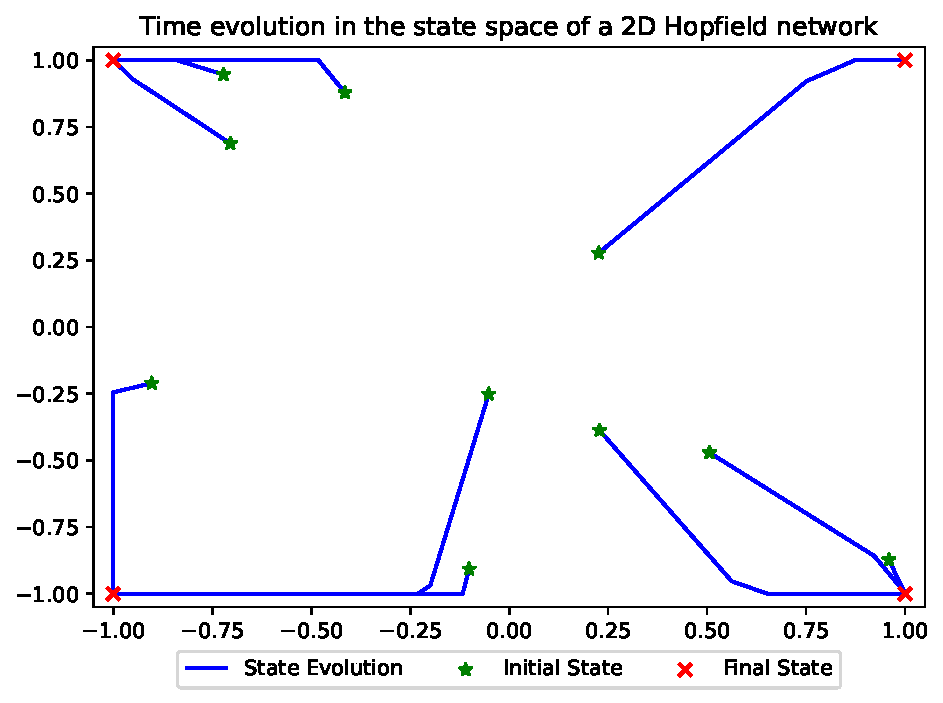
\includegraphics[width=\textwidth]{ex2_1_hopfield2D.pdf}
    \label{fig:ex2_1_hopfield2D}
  \end{subfigure}
  \begin{subfigure}{0.49\textwidth}
    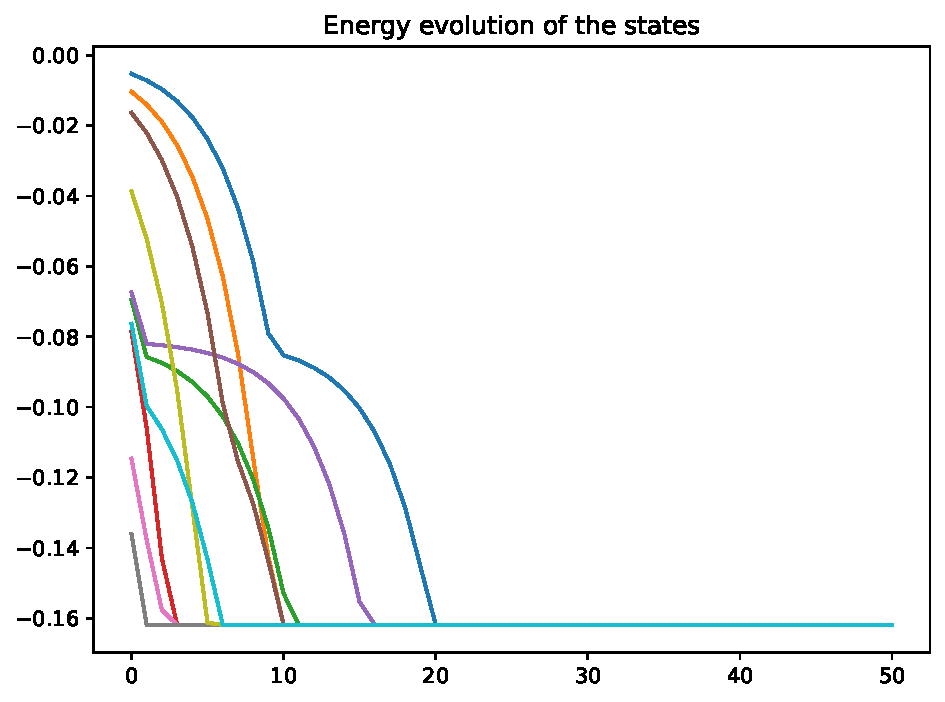
\includegraphics[width=\textwidth]{ex2_1_energy2D.pdf}
    \label{fig:ex2_1_energy2D}
  \end{subfigure}
  \caption{2D network: random inputs}
  \label{fig:ex2_1_2D_random}
\end{figure}

\begin{figure}[ht!]
  \centering
  \begin{subfigure}{0.49\textwidth}
    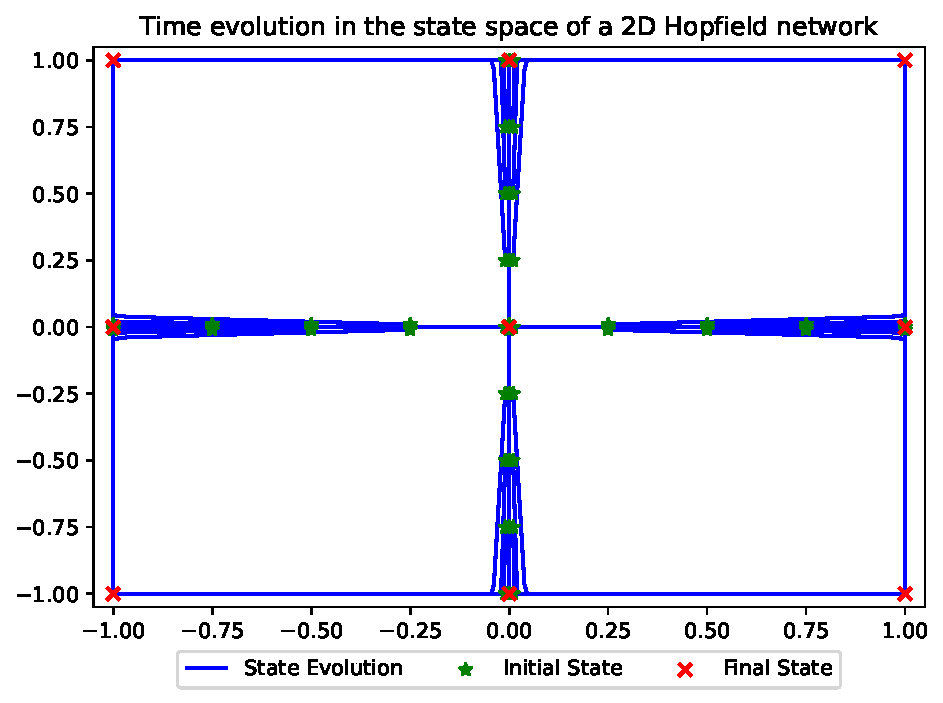
\includegraphics[width=\textwidth]{ex2_1_hopfield2D_edge.pdf}
    \label{fig:ex2_1_hopfield2D_edge}
  \end{subfigure}
  \begin{subfigure}{0.49\textwidth}
    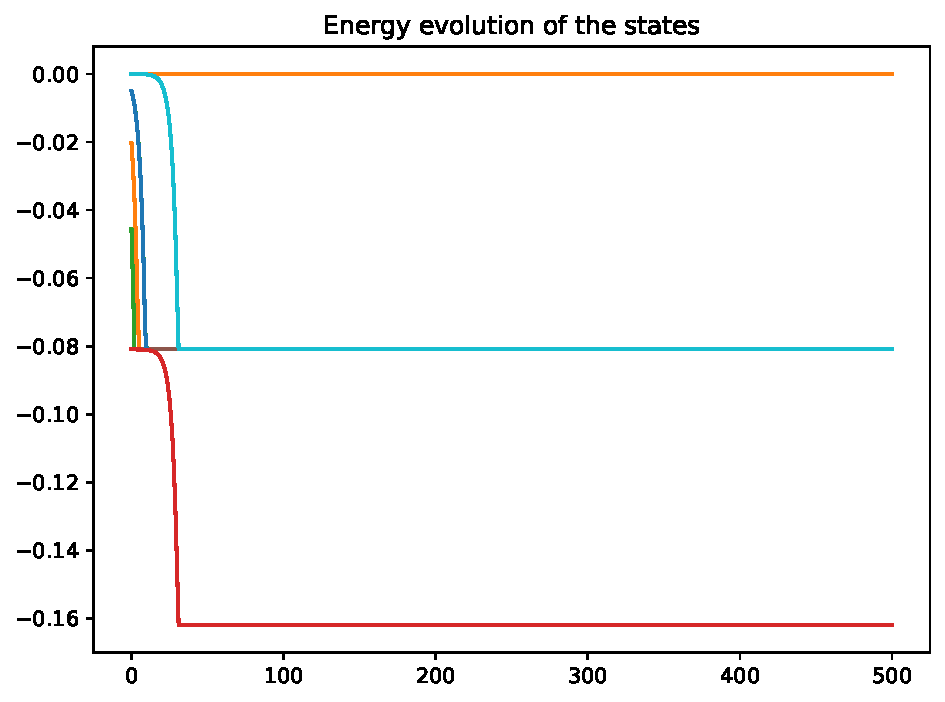
\includegraphics[width=\textwidth]{ex2_1_energy2D_edge.pdf}
    \label{fig:ex2_1_energy2D_edge}
  \end{subfigure}
  \caption{2D network: inputs close to local minima}
  \label{fig:ex2_1_2D_edge}
\end{figure}



\begin{task}{2.1.2}
  % Do the same for a three neuron Hopfield network, this time for the target patterns $[1, 1, 1]$,
  % $[-1, -1, 1]$ and $[1, -1, -1]$.
\end{task}

For the 3D network, all the target patterns $[1, 1, 1]$, $[-1, -1, 1]$ and $[1, -1, -1]$ are
reached, as shown in Figure~\ref{fig:ex2_1_3D_random}. No additional attractors are found. The
average number of iterations is $11.7$. All of the attractors are stable, even if the initial points
are placed exactly in the middle between two attractors, as shown in Figure~\ref{fig:ex2_1_3D_edge}.
The simulated points first move towards the plane that goes through all three attractors, and then
moves along this plane to the closest attractor.

\begin{figure}[ht!]
  \centering
  \begin{subfigure}{0.49\textwidth}
    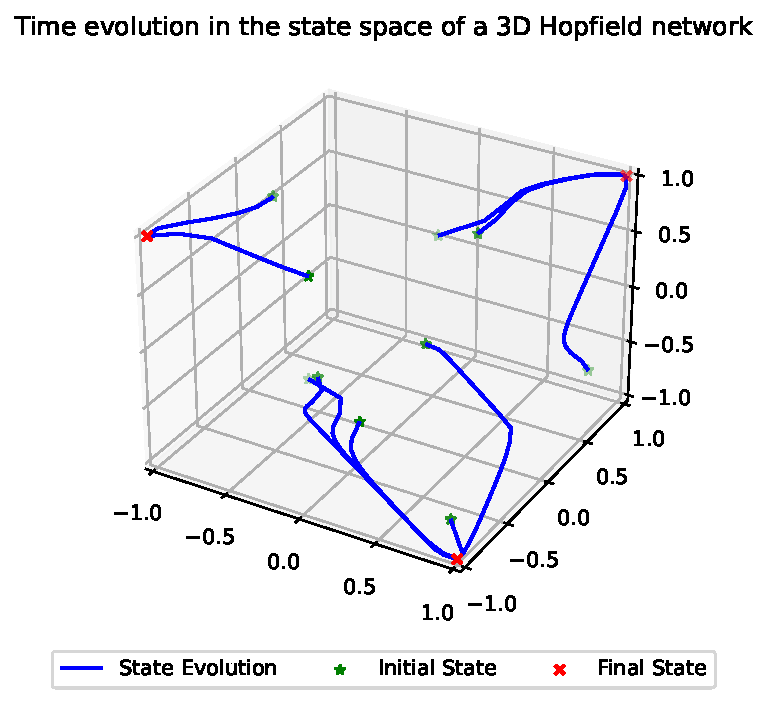
\includegraphics[width=\textwidth]{ex2_1_hopfield3D.pdf}
    \label{fig:ex2_1_hopfield3D}
  \end{subfigure}
  \begin{subfigure}{0.49\textwidth}
    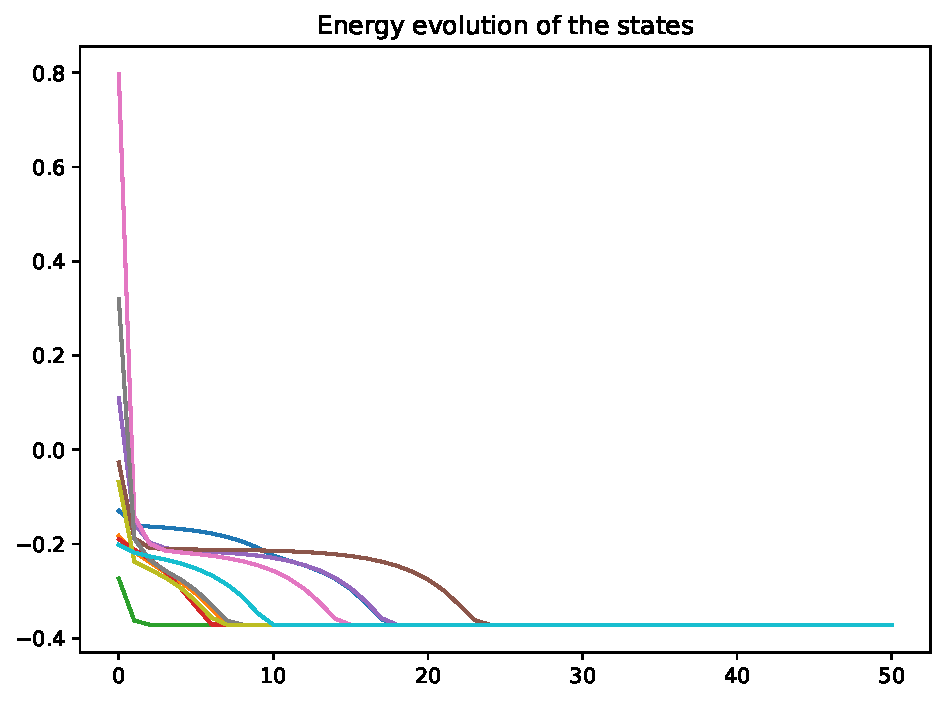
\includegraphics[width=\textwidth]{ex2_1_energy3D.pdf}
    \label{fig:ex2_1_energy3D}
  \end{subfigure}
  \caption{3D network: random inputs}
  \label{fig:ex2_1_3D_random}
\end{figure}

\begin{figure}[ht!]
  \centering
  \begin{subfigure}{0.49\textwidth}
    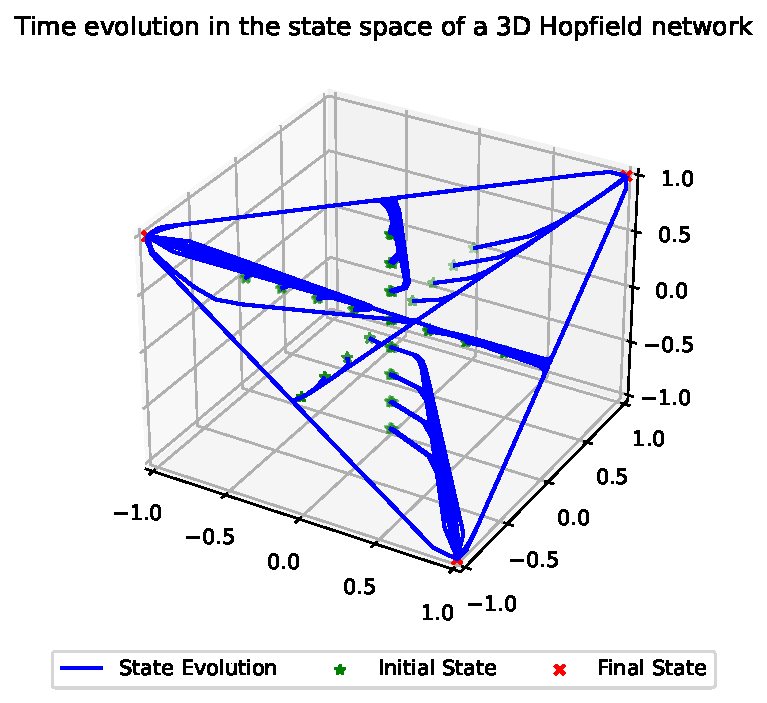
\includegraphics[width=\textwidth]{ex2_1_hopfield3D_edge.pdf}
    \label{fig:ex2_1_hopfield3D_edge}
  \end{subfigure}
  \begin{subfigure}{0.49\textwidth}
    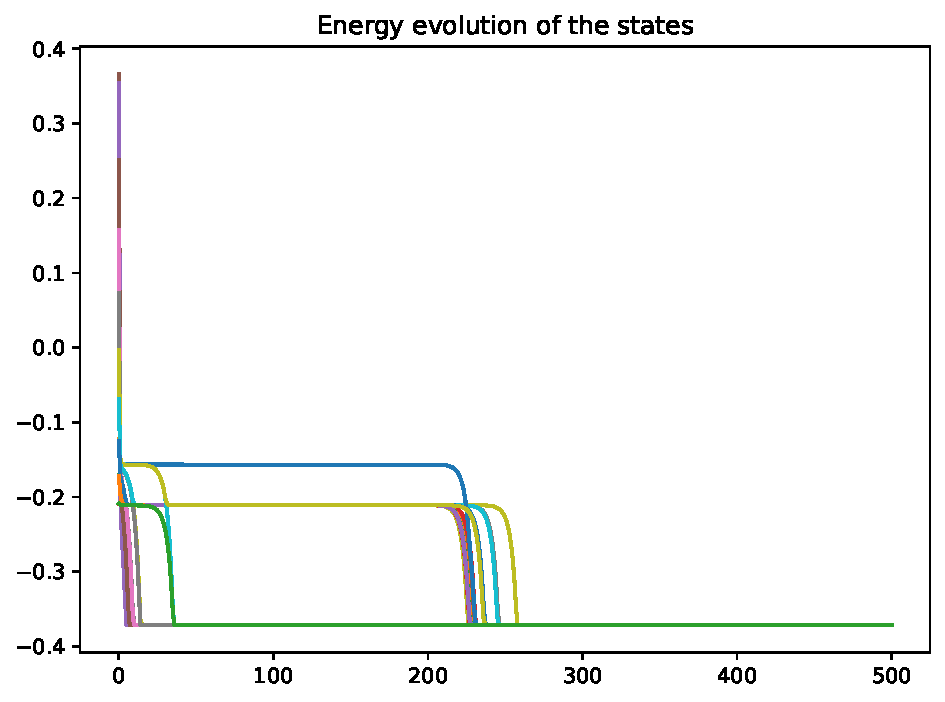
\includegraphics[width=\textwidth]{ex2_1_energy3D_edge.pdf}
    \label{fig:ex2_1_energy3D_edge}
  \end{subfigure}
  \caption{3D network: inputs close to local minima}
  \label{fig:ex2_1_3D_edge}
\end{figure}



\begin{task}{2.1.3}
  % Create a higher dimensional Hopfield network which has as attractors the handwritten digits from
  % 0 to 9. Test the ability of the network to correctly retrieve these patterns when some noisy
  % digits are given as input to the network. Try to answer the below questions by playing with
  % these two parameters:
  % \begin{itemize}
  %   \item \texttt{noise level} represents the level of noise that will corrupt the digits and is
  %         a positive number.
  %   \item \texttt{num iter} is the number of iterations the Hopfield network (having as input the
  %         noisy digits) will run.
  % \end{itemize}
  % Is the Hopfield model always able to reconstruct the noisy digits? If not why? What is the
  % influence of the noise on the number of iterations?
\end{task}

For $100$ iterations, the network is able to reconstruct the noisy digits for noise levels up to
$5$. Above this level, a few digits converge to the wrong attractor. Some digits are less robust to
noise than others. For example, the digit $7$ is often reconstructed as a $3$. Also, with less
iterations, the network often does not fully converge to an attractor. This leaves traces of the
noisy input in the reconstructed digit. For a good reconstruction with a noise level of $5$, the
number of iterations should be at least $40$. For a noise level of $1$, the network is able to
converge after only $4$ iterations.


\subsection{Timeseries Prediction}
\label{ex:2.2}


\begin{task}{2.2.1}
  % Train an MLP with one hidden layer. Investigate the model performance with different lags and
  % number of neurons. Discuss how the model looks and explain clearly how you tune the parameters
  % and what the influence on the final prediction is. Which combination of parameters gives the
  % best performance (MSE) on the test set?
\end{task}

The MLP model consists of an input layer with $lag = 80$ neurons, a hidden layer with $100$ neurons,
and an output layer with $1$ neuron. The model is trained for $3$ folds and $200$ epochs each. The
loss for each fold is shown in Figure~\ref{fig:ex2_2_mlp_loss}. The parameters were tuned based on
the loss on the validation set of size $150$. Using a bigger hidden layer and more lag improved the
performance the most. However, the model was overfitting a lot if there were too many validation
folds. Using fewer folds with a bigger hidden layer yielded better results than using more folds
with a smaller hidden layer. Also, the MSE on the test set would vary a lot between different
runs with the same parameters. This could be due to the initialization of the weights. The final
MSE on the test set was $277.3$ for $lag = 80$ and $100$ neurons in the hidden layer.

\begin{figure}[ht!]
  \centering
  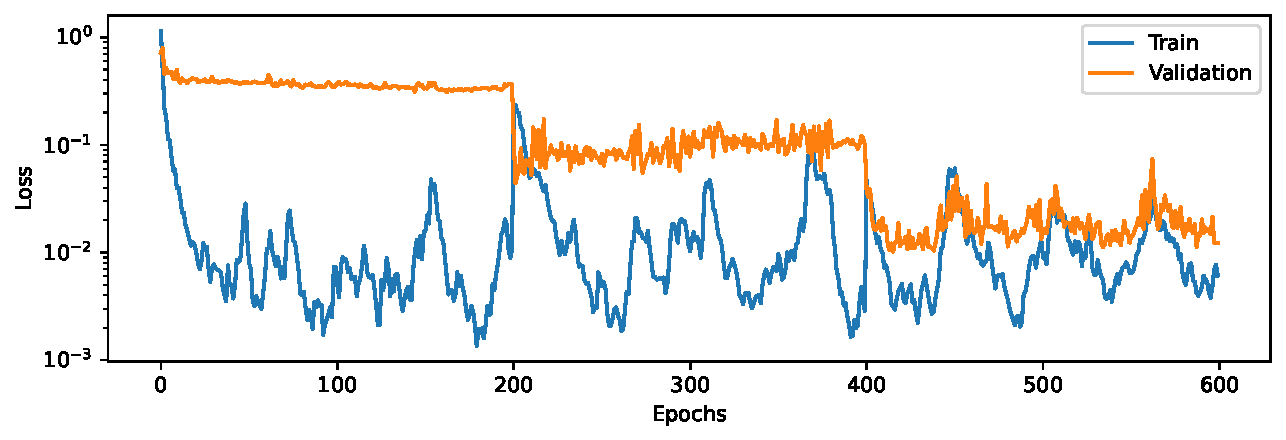
\includegraphics[width=0.9\textwidth]{ex2_2_mlp_loss.pdf}
  \caption{MLP loss for $3$ folds and $200$ epochs each.}
  \label{fig:ex2_2_mlp_loss}
\end{figure}



\begin{task}{2.2.2}
  % Do the same for the LSTM model and explain the design process. What is the effect of changing
  % the lag value for the LSTM network?
\end{task}

The LSTM model was also trained for $3$ folds, $lag = 80$ and $100$ neurons in the hidden layer, but
only for $150$ epochs. This was done to keep the results comparable to the MLP model. The parameters
were tuned based on the loss on the validation set of size $150$. The loss for each fold is shown in
Figure~\ref{fig:ex2_2_lstm_loss}, which still shows a small performance improvement for the third
fold. When using more folds, the performance of the LSTM model was decreasing. Using a lower lag
value also decreased the performance, which means that the LSTM model is able to capture a lot of
the temporal dependencies. The final MSE on the test set was $90.3$.

\begin{figure}[ht!]
  \centering
  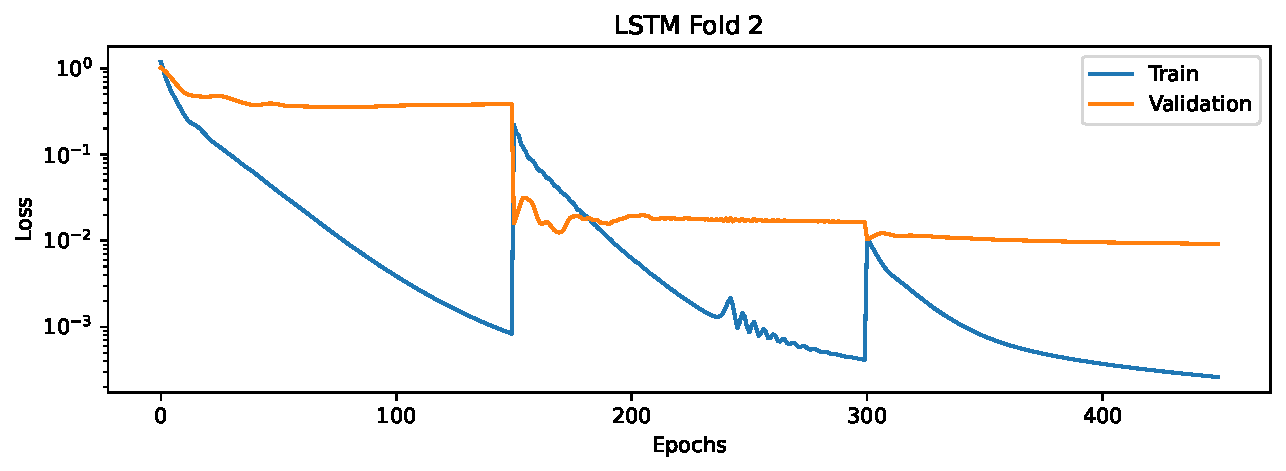
\includegraphics[width=0.9\textwidth]{ex2_2_lstm_loss.pdf}
  \caption{LSTM loss for $3$ folds and $150$ epochs each.}
  \label{fig:ex2_2_lstm_loss}
\end{figure}



\begin{task}{2.2.3}
  % Compare the results of the recurrent MLP with the LSTM. Which model do you prefer and why?
\end{task}

As shown in Figure~\ref{fig:ex2_2_comparison}, the LSTM model outperforms the MLP model. For the
first two thrids of the test set, the MLP and LSTM models predict the timeseries similarly. However,
after the regular pattern changes, the MLP model is not able to predict the timeseries well. This
could be due to the LSTM model being better at remembering and understanding the previous states of
the timeseries. This is also reflected in the lower MSE of the LSTM model. Therefore, the LSTM model
is preferred over the MLP model for this task.

\begin{figure}[ht!]
  \centering
  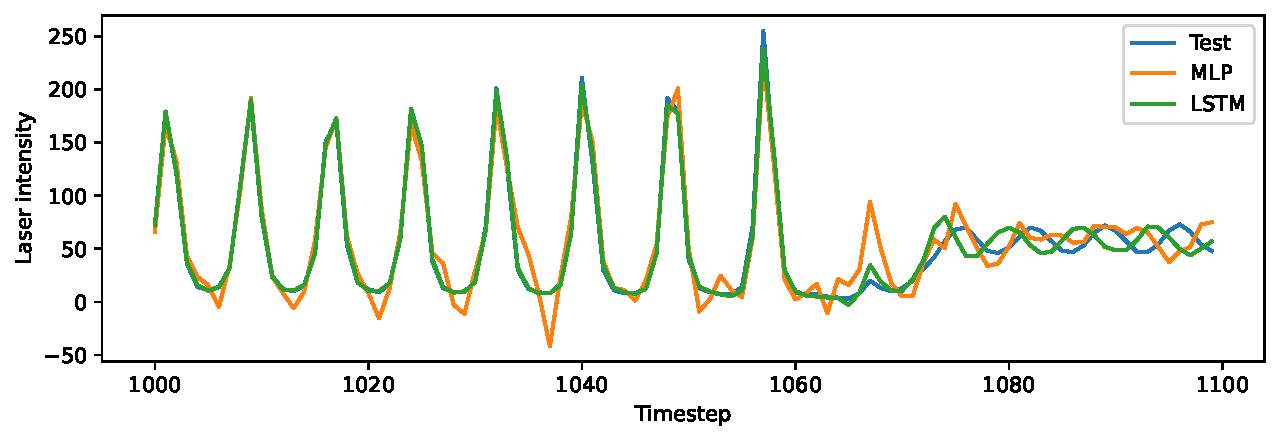
\includegraphics[width=0.9\textwidth]{ex2_2_comparison.pdf}
  \caption{Prediction results on continuation of the Santa Fe laser dataset.}
  \label{fig:ex2_2_comparison}
\end{figure}
